\chapter{Camara RGBD}
\label{chap:Camara RGBD}
\Abstract{En este anexo se desarrollará la conexión con la cámara RGBD Intel realsense L515 y las funcionalidades del driver desarrollado.}
Para el desarrollo de este proyecto se ha decidido emplear la cámara Intel Realsense L515 \citep{IntelL515} ya que dispone de todos los sensores necesarios, buenas prestaciones y un reducido coste. Para controlar la cámara se ha desarrollado un \textit{driver} para permitir la conexión directa a través de Python y el \textit{wrapper} desarrollado por Intel.

\begin{figure}[ht]
	\centering
	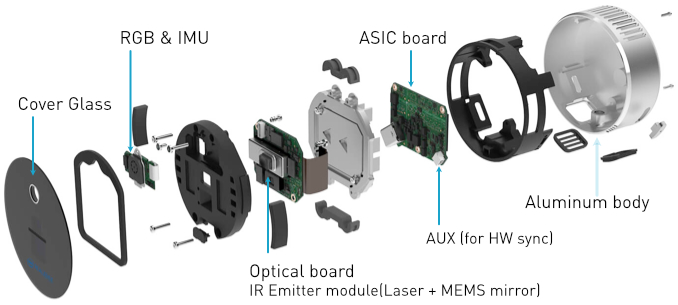
\includegraphics[width=0.95\textwidth]{Camara RGBD/l515_detailed.jpeg}
	\caption[Cámara Intel Realsense L515]{Cámara Intel Realsense L515 \citep{IntelL515}}
	\label{chap:Camara RGBD fig:camara}
\end{figure}

Para la conexión con la cámara se ha desarrollado una clase en Python de forma que el usuario pueda acceder a todas las funciones necesarias de forma cómoda y simple sin necesidad de entender como funciona internamente. La clase se encarga de establecer la conexión con la cámara y al crear nuestra clase en base al \textit{wrapper} desarrollado por Intel, nos permite tener acceso a todas las configuraciones y capacidades de la cámara y basarnos en estas para desarrollar una clase más simple e intuitiva de cara al usuario.

El \textit{driver} se ha desarrollado con varias funcionalidades en mente:
\begin{itemize}
\item Abstracción de la cámara: se desea que durante el desarrollo de las diferentes partes del proyecto no se deba de tener en cuenta la cámara y la configuración de la misma.
\item Independencia del \textit{hardware}: al emplear el mismo \textit{driver} en todas las partes del proyecto, se puede plantear en un futuro un cambio de cámara y el impacto en el proyecto será mínimo.
\item Calibración: el \textit{driver} debe de ser capaz de extraer todo el potencial de la cámara. Esto implica que se debe de añadir la funcionalidad de calibración tanto de las imágenes de color como de profundidad.
\item Alineación: La cámara L515 esta a su vez constituida por diferentes sensores con diferentes parámetros y configuraciones. Con el objetivo de poder relacionar las diferentes imágenes se debe de poder alinear correctamente todas las imágenes.
\end{itemize}

Uno de los puntos más importantes al desarrollar el \textit{driver} ha sido la capacidad de calibración. Al tratarse de diferentes sensores estos deben de estar bien calibrados con sus parámetros intrísecos bien definidos pero a su vez también se deben de definir la relación entre estos sensores con los parámetros extrínsicos. Para la calibración de la cámara de color se pueden emplear varios métodos pero e ha decidido optar por une de los más extendidos basado en la detección de patrones (tablero de ajedrez) con una distancia entre patrones predefinida. Por el contrario, la imagen de profundidad ha sido un mayor obstáculo debido al tipo de tecnología empleada. Al detectar distancias no es capaz de detectar el patrón y por lo tanto en una primera instancia no se puede emplear este método. Este obstáculo se ha conseguido solucionar empleando la imagen de infrarrojos. Esta se obtiene a través del mismo sensor (ambos emplean el sensor \textit{LiDAR}) y es capaz de distinguir el patrón.

\begin{figure}[ht]
  \subfloat{
	\begin{minipage}[c][1\width]{0.3\textwidth}
	   \centering
	   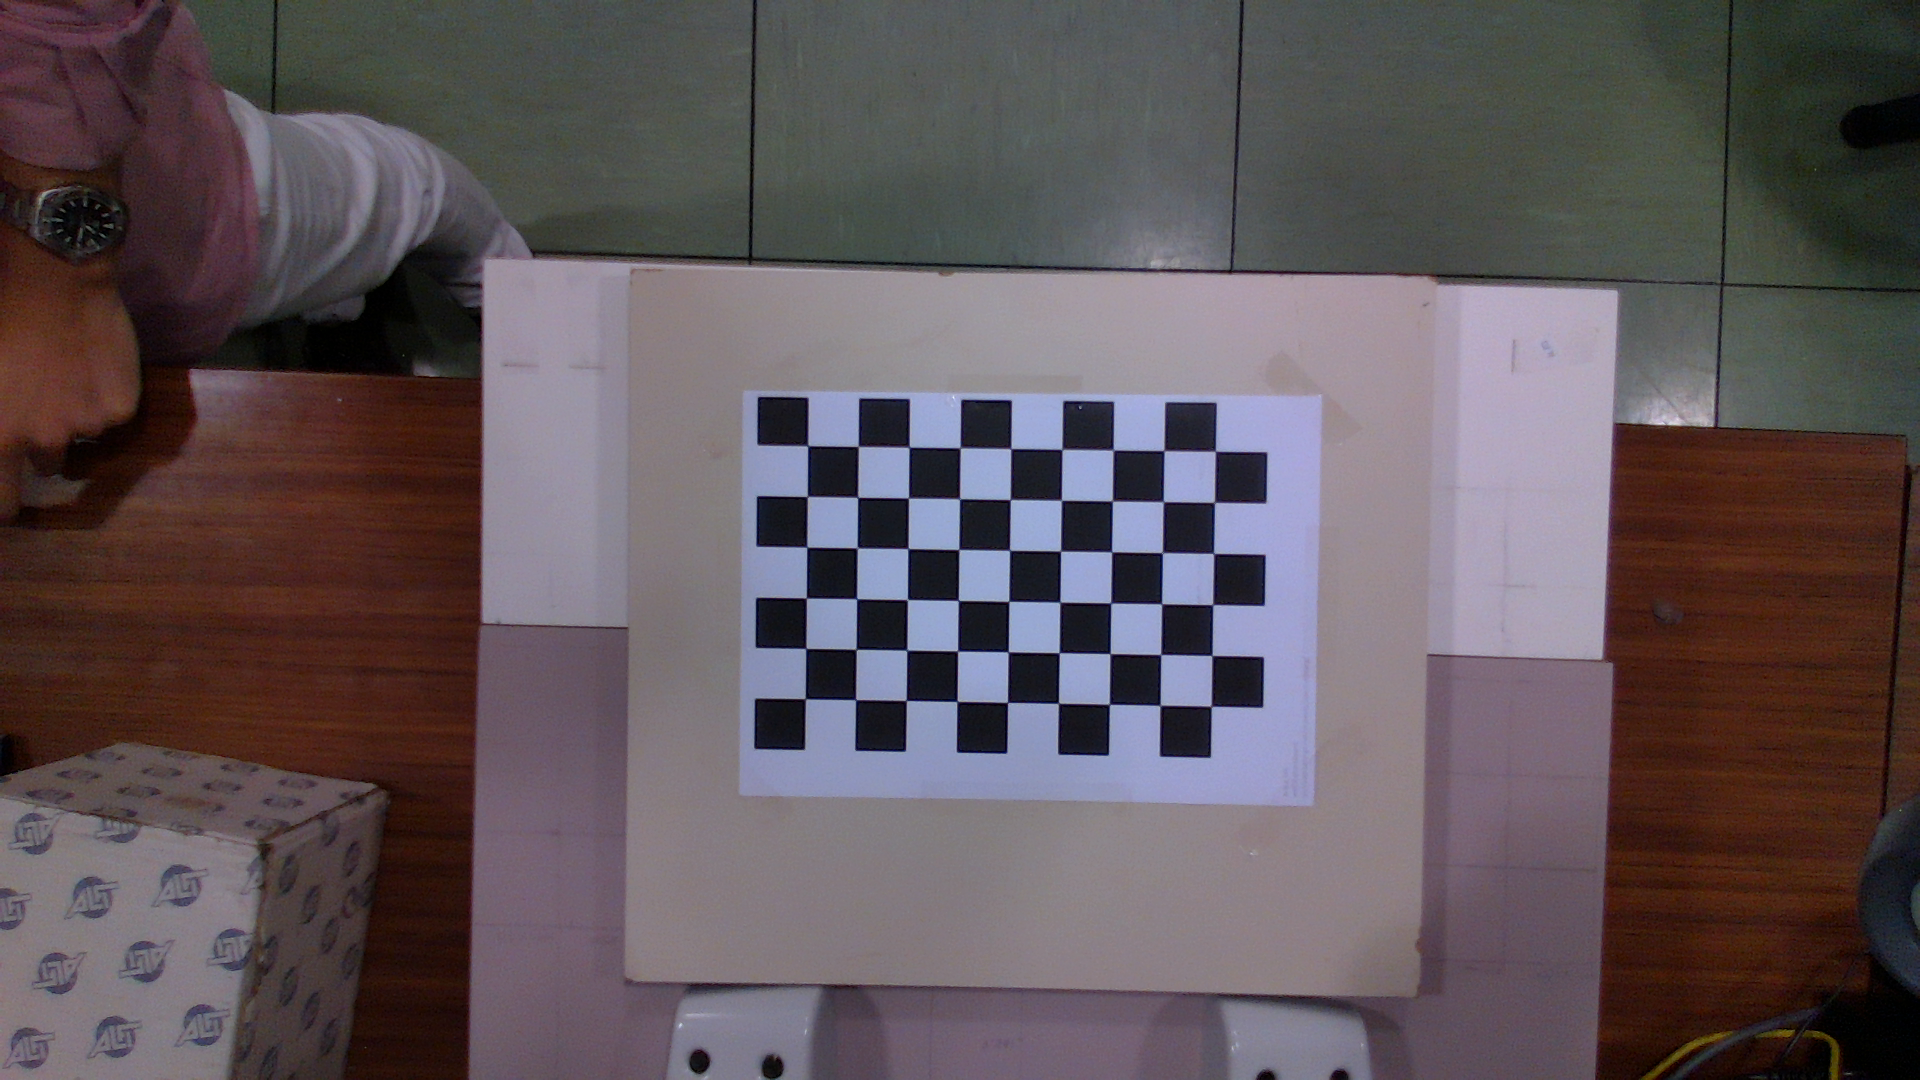
\includegraphics[width=1\textwidth]{Camara RGBD/0000_Colour.png}
	\end{minipage}}
  \hfill	
  \subfloat{
	\begin{minipage}[c][1\width]{0.3\textwidth}
	   \centering
	   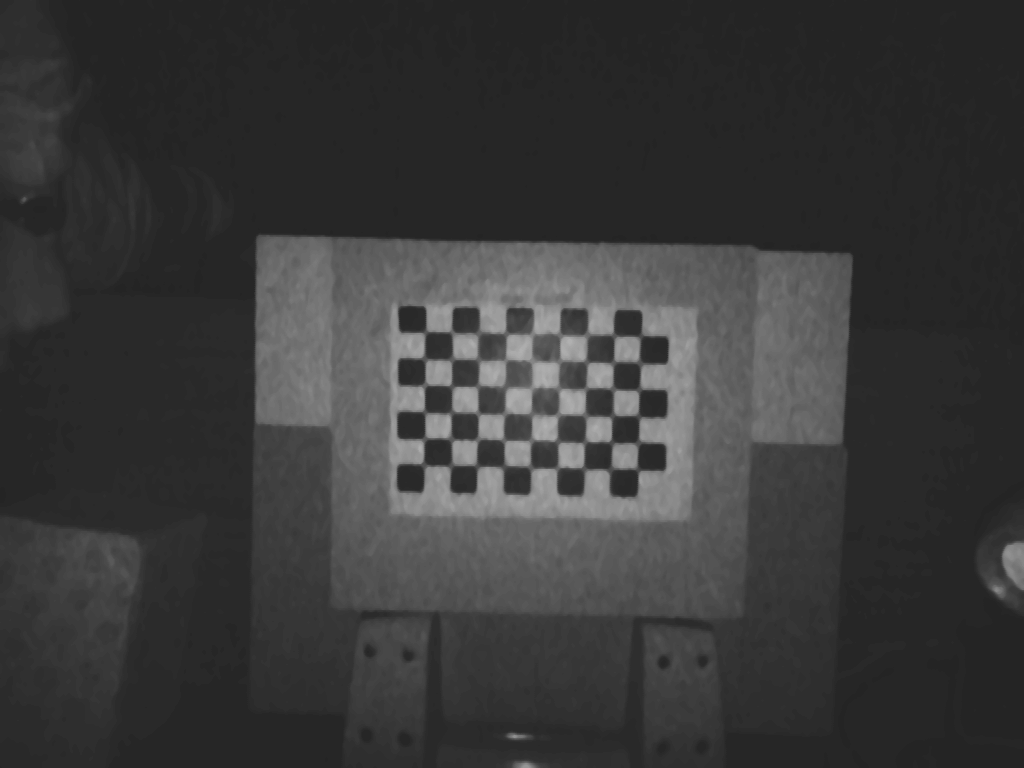
\includegraphics[width=1\textwidth]{Camara RGBD/0000_IR.png}
	\end{minipage}}
  \hfill	
  \subfloat{
	\begin{minipage}[c][1\width]{0.3\textwidth}
	   \centering
	   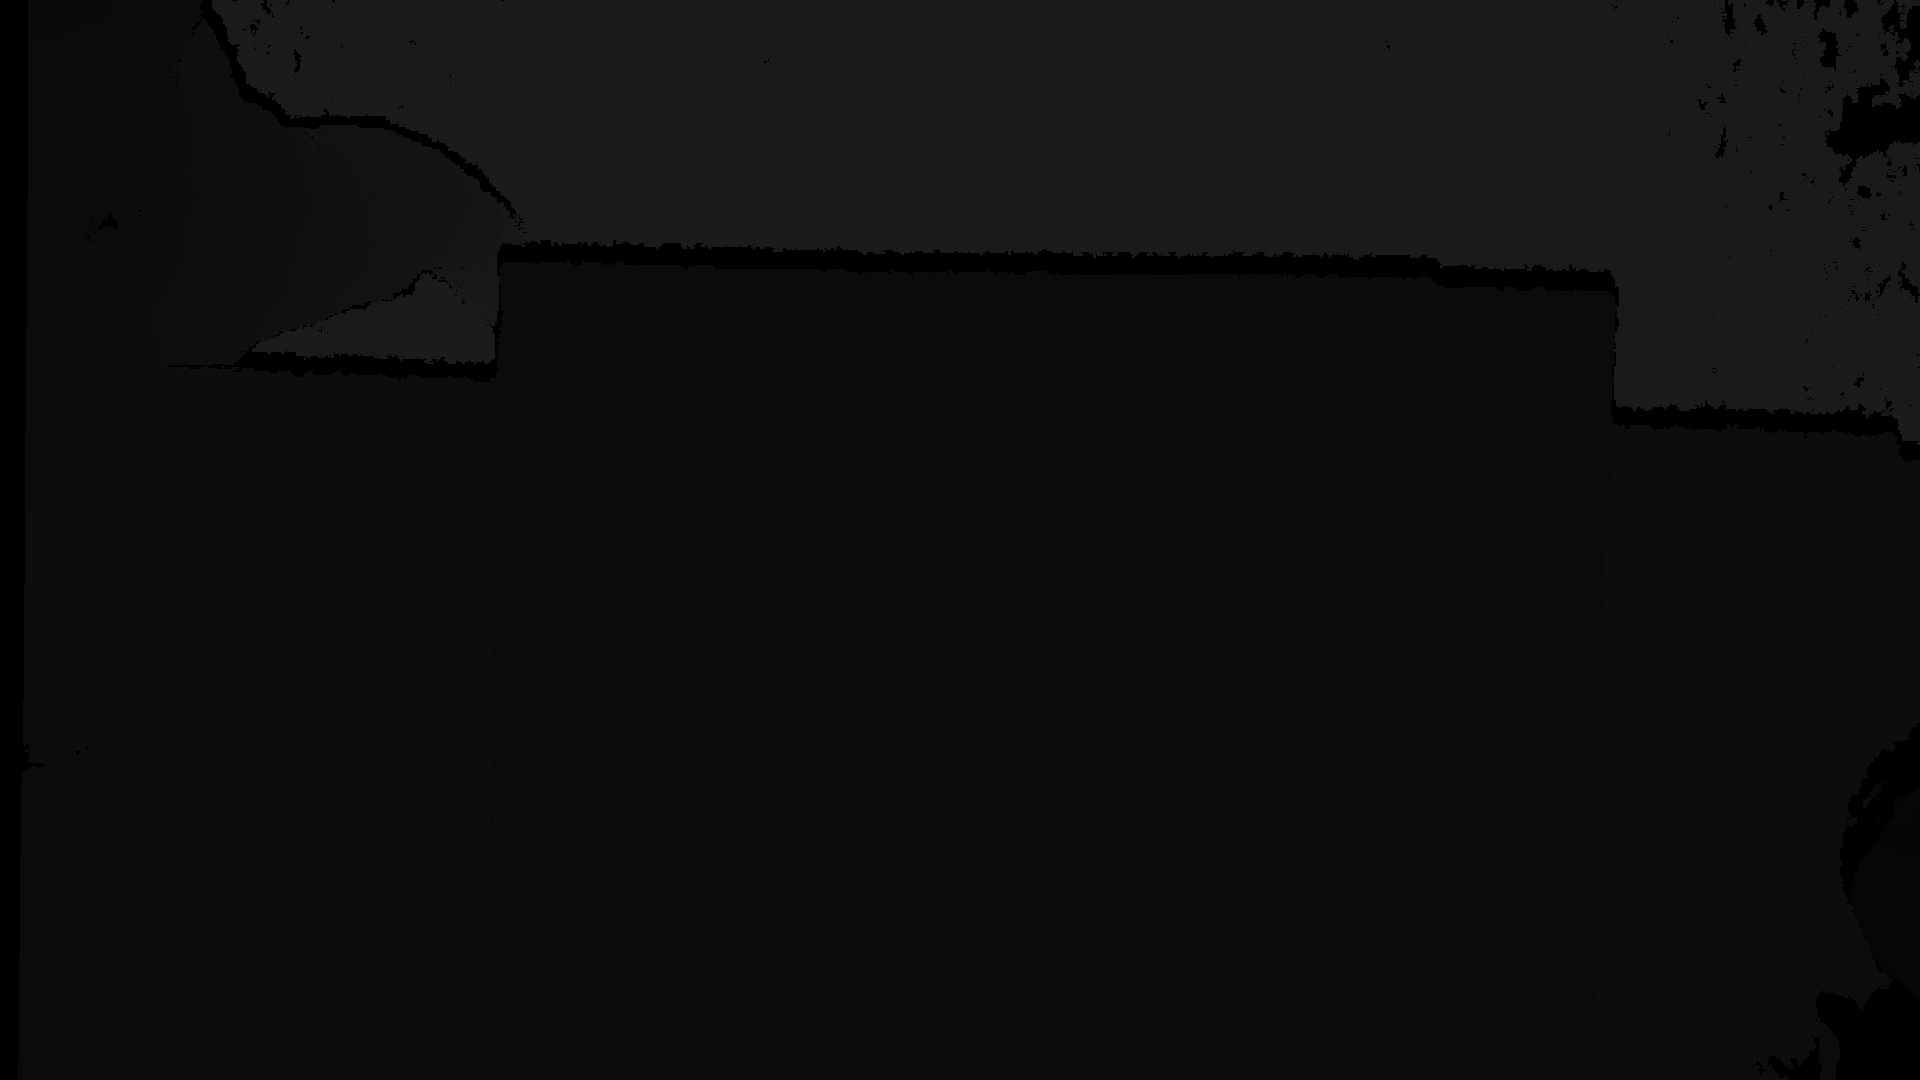
\includegraphics[width=1\textwidth]{Camara RGBD/0000_Depth.png}
	\end{minipage}}
\caption{Comparativa de imágenes de color, infrarrojos y profundidad con Realsense L515}
\label{chap:Camara RGBD fig: Comparativa sensores}
\end{figure}

Tras solucionar los problemas de calibración se ha podido desarrollar el \textit{driver} que tomará el control de la cámara y permitirá abstraer el resto del proyecto del \textit{hardware}. A continuación se muestra la funcionalidad del \textit{driver} desarrollado:

\begin{itemize}
\item Constructor: Se ha desarrollado un constructor personalizado que permite establecer la conexión con la cámara y establecer las opciones de funcionamiento.
\item Destructor: El destructor se ha desarrollado para que durante el proceso de destrucción de la instancia primero se corte de forma gradual la conexión con la cámara. De esta forma se evita futuros errores al intentar reconectarse a la cámara. Si no se realiza una desconexión progresiva no se podrá volver a abrir una conexión con la cámara y será necesario desconectar la cámara o reiniciar el \textit{driver}.
\item setCalibration: Carga y aplica los parámetros definidos por el proceso de calibración.
\item getColour: función para la captura solo de la imagen de color. Devuelve la imagen de color con una resolución de 1920x1080x3 píxeles
\item getDepth: función para la captura solo de la imagen de profundidad. Devuelve la imagen de con o sin alineamiento con la de color y con una resolución de 1024x768 píxeles.
\item getIR: función para la captura solo de la imagen de infrarrojos. Devuelve la imagen de con o sin alineamiento con la de color y con una resolución de 1024x768 píxeles.
\item getImages: Combina las anteriores funciones para obtener la salida de todos los sensores con una sola llamada.
\item saveImages: captura y guarda las imágenes obtenidas por todos los sensores.
\item transformRGBToDepth: relaciona puntos de la imagen de color con la imagen de profundidad (imagen no alineada).
\item getPosition: relaciona un punto en pixeles con sus coordenadas en el mundo real.
\end{itemize}

\begin{figure}[ht]
  \subfloat{
	\begin{minipage}[c][1\width]{0.3\textwidth}
	   \centering
	   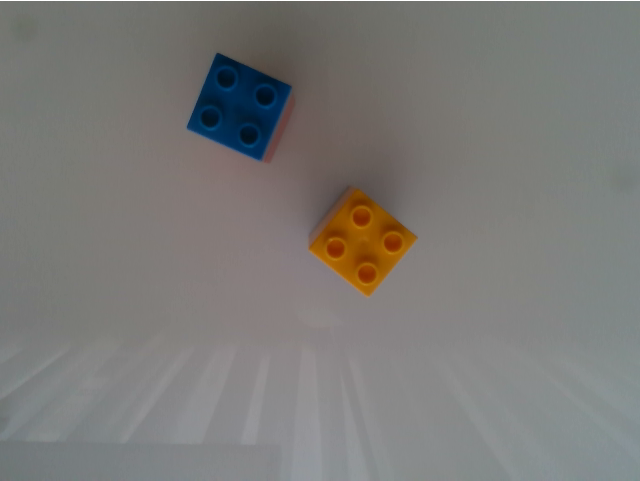
\includegraphics[width=1\textwidth]{Camara RGBD/color.png}
	\end{minipage}}
  \hfill	
  \subfloat{
	\begin{minipage}[c][1\width]{0.3\textwidth}
	   \centering
	   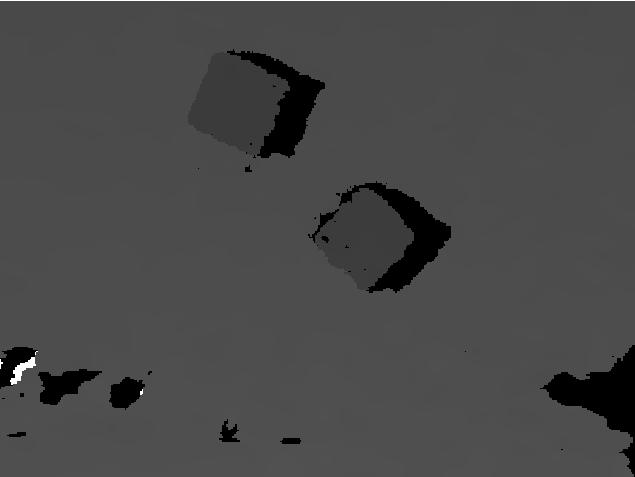
\includegraphics[width=1\textwidth]{Camara RGBD/con ajuste.png}
	\end{minipage}}
  \hfill	
  \subfloat{
	\begin{minipage}[c][1\width]{0.3\textwidth}
	   \centering
	   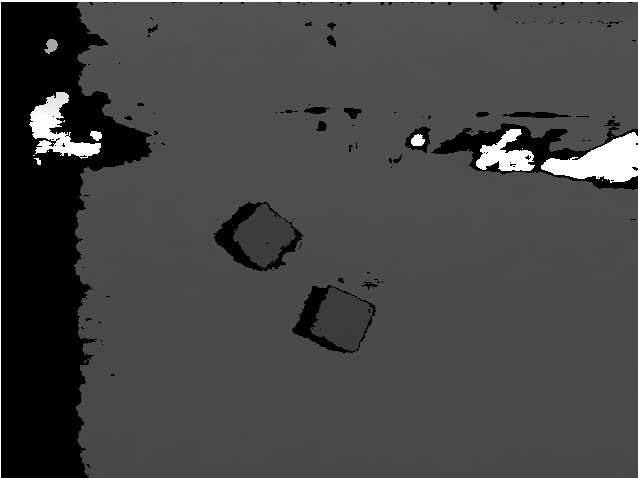
\includegraphics[width=1\textwidth]{Camara RGBD/sin ajuste.png}
	\end{minipage}}
\caption[Alineamiento de imágenes de color y profundidad]{Alineamiento de las imágenes de color y profundidad tomadas con la cámara Realsense L515}
\label{chap:Camara RGBD fig: Alineamiento}
\end{figure}